\section{El Espacio Euclídeo. Espacios normados y métricos.}

\begin{ejercicio}
    Probar que, en cualquier espacio pre-hilbertiano $X$, el producto escalar se obtiene a partir de la norma mediante la llamada \emph{identidad de polarización}:
    \begin{equation*}
        4(x|y)=\left\lVert x+y \right\rVert^{2} - \left\lVert x-y \right\rVert^{2} \quad \forall x,y \in X 
    \end{equation*}

    Se tiene que:
    \begin{multline*}
        ||x+y||^2 - ||x-y||^2 = (x+y|x+y) - (x-y|x-y) =\\=
        \cancel{(x|x)} + (x|y) + (y|x) + \bcancel{(y|y)} - \cancel{(x|x)} + (x|y) + (y|x) - \bcancel{(y|y)} = 4(x|y)
    \end{multline*}
    donde he usado que $(x|y)=(y|x)$ por ser simétrica, y que $||x||=\sqrt{(x|x)}$.
\end{ejercicio}

\begin{ejercicio}
     Si $X$ e $Y$ son espacios pre-hilbertianos, es una sana costumbre denotar ambos productos escalares por $(\cdot|\cdot)$ y ambas normas asociadas por $||\cdot ||$. Sea $f : X \to Y$ una aplicación lineal que preserva la norma, es decir,
     \begin{equation*}
        \left\lVert f(x) \right\rVert = \left\lVert x \right\rVert
    \end{equation*}

    Probar que entonces $f$ también preserva el producto escalar:
    \begin{equation*}
        \left( f(x) \ | \ f(y) \right) = (x|y) \quad \forall  x,y \in X
    \end{equation*}

    Tenemos que:
    \begin{multline*}
        4(x|y)
        \AstIg ||x+y||^2 - ||x-y||^2
        = ||f(x+y)||^2 - ||f(x-y)||^2
        = ||f(x)+f(y)||^2 - ||f(x)-f(y)||^2
        =\\\AstIg 4(f(x)|f(y)) \Longrightarrow (x|y)=(f(x)|f(y))
    \end{multline*}
    donde en $(\ast)$ he aplicado el ejercicio anterior; y he aplicado que por ser $f$ una aplicación lineal se tiene que $f(x+y)=f(x)+f(y)$.
\end{ejercicio}


\begin{ejercicio}
    Probar que todo espacio pre-hilbertiano $X$ de dimensión $N \in \bb{N}$, se identifica totalmente con el espacio euclídeo $N$-dimensional; es decir, existe una biyección lineal $f : X \to \bb{R}^{N}$ que preserva el producto escalar:
    \begin{equation*}
        \left(f(x)|f(y)\right)=(x|y) \quad \forall x,y \in X
    \end{equation*}

    En este sentido podemos decir que el espacio euclídeo $N$-dimensional es el único espacio pre-hilbertiano de dimensión $N$.\\

    Sea $\cc{B}_X$ una base ortonormal de $X$, y $\cc{B}_{\bb{R}}$ una base ortonormal de $\bb{R}^N$.
    \begin{equation*}
        \cc{B}_X=\{v_1,\dots, v_n\}
        \hspace{1cm}
        \cc{B}_{\bb{R}}=\{e_1,\dots, e_n\}
    \end{equation*}

    Entonces, definimos $f:X\to \bb{R}^N$ forma lineal de forma que los vectores de una base de aplican en los de la otra base. Es decir, $f(v_i)=e_i, \quad \forall i=1,\dots, n$. Como es una forma lineal y se aplica base en otra base, tenemos que es una biyección lineal.\\
    
    Sea $x, y\in X$ tal que $x=\sum\limits_{i=1}^n a_iv_i,~ y=\sum\limits_{i=1}^n b_iv_i$. Comprobemos que preserva el producto escalar. 
    \begin{multline*}
        \left(f(x)|f(y)\right)
        = \left(f\left(\sum_{i=1}^n a_iv_i\right)\left|~f\left(\sum_{i=1}^n b_iv_i\right)\right.\right)
        = \left(\sum_{i=1}^n a_if\left(v_i\right)\left|~\sum_{i=1}^n b_if\left(v_i\right)\right.\right) =\\
        = \left(\sum_{i=1}^n a_ie_i\left|~\sum_{i=1}^n b_ie_i\right.\right)
        \AstIg \sum_{i=1}^n a_ib_i
        \AstIg \left(\sum_{i=1}^n a_iv_i\left|~\sum_{i=1}^n b_iv_i\right.\right)
        = (x|y)
    \end{multline*}
    donde en $(\ast)$ he aplicado que las bases escogidas son ortonormales, por lo que el producto escalar de dos elementos es la suma del producto de sus componentes expresadas en la correspondiente base.
\end{ejercicio}


\begin{ejercicio}
    Probar que, en todo espacio pre-hilbertiano $X$, se verifica la \emph{identidad del paralelogramo}:
    \begin{equation*}
        \left\lVert x+y \right\rVert^{2} + \left\lVert x-y \right\rVert^{2}
        = 2\left\lVert x \right\rVert^{2} + 2\left\lVert y \right\rVert^{2} \quad \forall x,y \in X
    \end{equation*}

    Interpretar geométricamente el resultado.

    \begin{equation*}
        ||x+y||^2 + ||x-y||^2 = ||x||^2 + ||y||^2 + 2(x|y) + ||x||^2 + ||y||^2 - 2(x|y) = 2||x||^2 + 2||y||^2
    \end{equation*}
    Geométricamente, tenemos que la suma de los cuadrados de los lados de un paralelogramo equivale a la suma de los cuadrados de las diagonales.
    \begin{figure}[H]
        \centering
        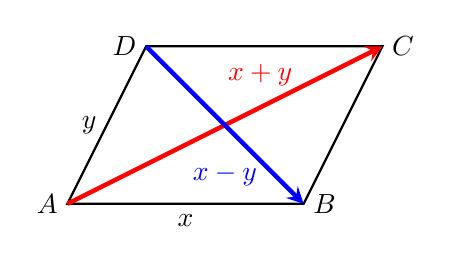
\begin{tikzpicture}
            % Coordenadas de los vértices del paralelogramo
            \coordinate (A) at (0,0);
            \coordinate (B) at (3,0);
            \coordinate (C) at (4,2);
            \coordinate (D) at (1,2);
            
            % Dibuja el paralelogramo
            \draw[thick] (A) -- node[below]{$x$}(B) -- (C) -- (D) -- node[left]{$y$} cycle;
            
            % Etiqueta los vértices
            \node[left] at (A) {$A$};
            \node[right] at (B) {$B$};
            \node[right] at (C) {$C$};
            \node[left] at (D) {$D$};
            
            % Dibuja las diagonales y etiquétalas
            \draw[-stealth, red, ultra thick] (A) -- node[above right, yshift=+10pt, xshift=-3pt] {$x+y$} (C);
            \draw[stealth-, blue, ultra thick] (B) -- node[below, yshift=-10pt] {$x-y$} (D);
        \end{tikzpicture}
    \end{figure}
\end{ejercicio}

\begin{ejercicio}
    Para cualquier espacio pre-hilbertiano $X$, discutir la posibilidad de que la desigualdad triangular sea una igualdad, es decir, encontrar la condición necesaria y suficiente que deben cumplir dos vectores $x, y \in X$ para verificar que $|| x + y|| =|| x|| + ||y||$.\\

    La demostración de la desigualdad triangular parte de la desigualdad de Cauchy-Schwartz: $$||(x|y)|| \leq ||x||~||y|| \qquad \forall x,y\in X$$
    Además, tenemos que la igualdad se da solo en el caso de que sean linealmente dependientes.

    Demostramos ahora la desigualdad triangular a partir de la desigualdad de Cauchy-Schwarz:
    \begin{multline*}
        ||x+y||^2 = ||x||^2 + ||y||^2 + 2(x|y) \stackrel{(1)}{\leq}
        ||x||^2 + ||y||^2 + 2|(x|y)| \stackrel{(2)}{\leq} \\
        \stackrel{(2)}{\leq}
        ||x||^2 + ||y||^2 + 2||x||~||y|| = \left(||x|| + ||y||\right)^2
    \end{multline*}
    
    
    Por tanto, tenemos que se da la igualdad si y solo si se dan las igualdades en $(1)$ y $(2)$.
    \begin{itemize}
        \item La igualdad en $(1)$ se da si y solo si $(x|y)\geq 0$.
        \item La igualdad en $(2)$ se da si y solo si se da la da desigualdad en Cauchy-Schwarz; y esta se da si y solo si $\{x,y\}$ son linealmente dependientes.
    \end{itemize}
    
    Por tanto, tenemos que se da la igualdad si y solo si ambos vectores son linealmente dependientes y además su producto escalar es positivo.
\end{ejercicio}

\begin{ejercicio}
    Discutir la posibilidad de que la desigualdad triangular para la norma de la suma en $\bb{R}^N$ sea una igualdad, es decir, encontrar la condición necesaria y suficiente que deben cumplir dos vectores $x, y \in \bb{R}^N$ para verificar la siguiente igualdad: $ ||x + y||_1 =|| x||_1 +|| y||_1$.\\

    En primer lugar, como la norma 1 no procede de ningún producto escalar, tenemos que no son aplicables los resultados del ejercicio anterior. Demostramos por tanto la desigualdad triangular en el caso de la norma 1:
    \begin{equation*}
        ||x+y||_1 = \sum_{k=1}^N |x_k + y_k| \leq \sum_{k=1}^N |x_k| + |y_k| = ||x||_1 + ||y||_2, \hspace{1cm} \forall x,y\in \bb{R}^n
    \end{equation*}

    Por tanto, tenemos que se dará la igualdad triangular si y solo si se cumple que $|x_k + y_k| = |x_k| + |y_k|,~\forall k\in \Delta_N$. Para que esto ocurra, es necesario y suficiente lo siguiente: $$x_k, y_k\geq 0,\hspace{1cm} \forall k\in \Delta_N$$
\end{ejercicio}

\begin{ejercicio}
    Probar que, para $N > 1$ , no existe un producto escalar en $\bb{R}^N$ cuya norma asociada sea la de la suma, y que lo mismo le ocurre a la norma del máximo. Probar también que, en el espacio vectorial $\cc{C}[0, 1]$~, las normas $|| \cdot ||_1 $ y $|| \cdot ||_\infty $ no son las asociadas a ningún producto escalar.\\

    Tenemos que en todo espacio pre-hilbertiano $X$ se cumple la identidad del paralelogramo:
    \begin{equation*}
        2||x||^2 + 2||y||^2 = ||x+y||^2 + ||x-y||^2, \hspace{1cm} \forall x,y\in X
    \end{equation*}
    
    Busquemos contraejemplos que demuestren que eso no es cierto para $X=\bb{R}^n$ con la norma 1 y la del máximo. Sean los valores siguientes:
    \begin{align*}
        x=(1,\dots, 1) && x+y = (0,2,\dots, 2) \\
        y=(-1,1,\dots, 1) && x-y = (2, 0, \dots, 0) 
    \end{align*}
    
    Veamos que no se cumple la identidad del paralelogramo en $\bb{R}^n$ para la norma 1 y el máximo:
    \begin{gather*}
        2||x||_1^2 + 2||y||_1^2 = 2n^2 + 2n^2 = 4n^2 \neq 
        [2(n-1)]^2 + 2^2 = ||x+y||_1^2 + ||x-y||_1^2 \\
        2||x||_\infty^2 + 2||y||_\infty^2 = 2\cdot 1^2 + 2\cdot 1^2 = 4 \neq 
        8= 2^2 + 2^2 = ||x+y||_\infty^2 + ||x-y||_\infty^2
    \end{gather*}

    Por tanto, en $\bb{R}^n$ con la norma 1 y la norma del máximo no se cumple la identidad del paralelogramo. Por tanto, no existe un producto escalar asociado a dichas normas.\\

    Veámoslo para el caso de $\cc{C}[0, 1]$. Sean los valores siguientes:
    \begin{align*}
        f(x)=\cos x\geq 0\in [0,1]~ &&& (f+g)(x)=\cos x + \sen x\geq 0 \in [0,1] \\
        g(x)=\sen x\geq 0\in [0,1] &&& (f-g)(x)=\cos x - \sen x
    \end{align*}

    Veámoslo para el caso de la norma 1:
    \begin{gather*}
        ||f||_1 = \int_0^1 |\cos x|~dx = \left.\sen x\right]_0^1 = \sen 1 \qquad
        ||g||_1 = \int_0^1 |\sen x|~dx = \left.-\cos x\right]_0^1 = -\cos 1 +1 \\
        ||f+g||_1 = \int_0^1 |\sen x +\cos x|~dx = \left.\sen x -\cos x\right]_0^1 = \sen 1 -\cos 1 +1
    \end{gather*}
    \begin{equation*}
        \begin{split}
            ||f-g||_1 &= \int_0^1 |\cos x -\sen x|~dx =\int_0^{\frac{\pi}{4}} \cos x -\sen x~dx + \int_{\frac{\pi}{4}}^1 \sen x -\cos x~dx =\\
            &= \left.\sen x +\cos x\right]_0^{\frac{\pi}{4}} + \left[-\cos x -\sen x\right]_{\frac{\pi}{4}}^1 = \sqrt{2}-1-\cos 1 -\sen 1+\sqrt{2}
        \end{split}
    \end{equation*}

    Escribimos ahora la identidad del paralelogramo para la norma 1:
    \begin{multline*}
        2||f||_1^2 + 2||g||_1^2 = 2\cdot \sen^2 1 +2\cdot (1-\cos 1)^2  \neq \\ \neq
        (1+\sen 1 -\cos 1)^2 + (2\sqrt{2}-1-\cos 1 -\sen 1)^2 = ||f+g||_1^2 + ||f-g||_1^2
    \end{multline*}

    Por tanto, en $\cc{C}[0,1]$ con la norma 1 no se cumple la identidad del paralelogramo; por lo que no existe un producto escalar asociado a dicha norma. Veámoslo para la norma del máximo.
    \begin{gather*}
        ||f||_\infty = \max_{x\in [0,1]}\{\cos x\} = 1 \qquad
        ||g||_\infty = \max_{x\in [0,1]}\{\sen x\} = \sen 1 \\
        ||f+g||_\infty = \max_{x\in [0,1]}\{\cos x + \sen x\} = (f+g)\left(\frac{\pi}{4}\right)=\sqrt{2} \\
        ||f-g||_\infty = \max_{x\in [0,1]}\{|\cos x - \sen x|\} = 1
    \end{gather*}
    Escribimos ahora la identidad del paralelogramo para la norma del máximo:
    \begin{equation*}
        2||f||_\infty^2 + 2||g||_\infty^2 = 2(1+\sen^2 1)  \neq 3=
        2 + 1^2 = ||f+g||_\infty^2 + ||f-g||_\infty^2
    \end{equation*}
    Por tanto, en $\cc{C}[0,1]$ con la norma del máximo no se cumple la identidad del paralelogramo; por lo que no existe un producto escalar asociado a dicha norma.
\end{ejercicio}

\begin{ejercicio}
    Sea $X$ un espacio vectorial y sean $\mu , \nu : X \to \bb{R} 
    $ dos normas en $X$. En cada uno de los siguientes casos, probar que la función $\left\lVert \cdot \right\rVert  : X \rightarrow \bb{R}$ , definida para todo $x \in X$ en la forma que se indica, es una norma en $X$:
    \begin{enumerate}
        \item $\left\lVert x \right\rVert = \mu (x) + \nu(x)$:

        Comprobamos las tres condiciones:
        \begin{itemize}
            \item $\left\lVert x \right\rVert = \mu (x) + \nu(x)\geq 0$ por ser la suma de términos no-negativos. Además, se tiene que $||x||=0\Longleftrightarrow \mu(x)=\nu(x)=0\Longleftrightarrow x=0$.

            \item $||\lambda x|| = \mu(\lambda x) + \nu(\lambda x) = |\lambda|~[\mu(x)+\nu(x)] = |\lm|~||x||$.

            \item $||x+y|| = \mu(x+y) + \nu(x+y)\leq \mu(x)+\nu(x) + \mu(y)+\nu(y)=||x|| + ||y||$.
        \end{itemize}
        
        \item $\left\lVert x \right\rVert = \max \{ \mu (x) , \nu(x) \}$

        Comprobamos las tres condiciones:
        \begin{itemize}
            \item $\left\lVert x \right\rVert = \max\{\mu(x),\nu(x)\}\geq 0$ por ser $\mu(x), \nu(x)\geq 0$. Además, se tiene que $||x||=0\Longleftrightarrow \mu(x)=\nu(x)=0\Longleftrightarrow x=0$.

            \item $||\lambda x|| = \max\{\mu(\lm x),\nu(\lm x)\}
            = \max\{|\lm |~\mu(x),|\lm |~\nu(x)\} 
            = |\lm |~\max\{\mu(x),\nu(x)\}$ y, por la definición de la norma, $|\lm|~||x||$.

            \item Probamos la desigualdad triangular:
            \begin{equation*}
                \begin{split}
                    ||x+y||
                    =& \max\{\mu(x+y),\nu(x+y)\}
                    \leq \max\{\mu(x)+\mu(y), \nu(x)+\nu(y)\} \stackrel{(\ast)}{\leq}\\
                    \stackrel{(\ast)}{\leq}& \max\{\mu(x), \nu(x)\} + \max\{\mu(y), \nu(y)\}
                    = ||x||+||y||
                \end{split}
            \end{equation*}
            donde en $(\ast)$ he aplicado lo siguiente:
            \begin{gather*}
                \mu(x)+\mu(y) \leq \max\{\mu(x), \nu(x)\} + \max\{\mu(y), \nu(y)\} \\
                \nu(x)+\nu(y) \leq \max\{\mu(x), \nu(x)\} + \max\{\mu(y), \nu(y)\}
            \end{gather*}
            
            
        \end{itemize}
        \item $\left\lVert x \right\rVert = \left[\mu (x)^{2} + \nu(x)^2\right]^{1/2}$
        
        Comprobamos las tres condiciones:
        \begin{itemize}
            \item $\left\lVert x \right\rVert =  \left[\mu (x)^{2} + \nu(x)^2\right]^{1/2}\geq 0$ por ser raíz de la suma de términos no-negativos. Además, se tiene que $||x||=0\Longleftrightarrow \mu(x)=\nu(x)=0\Longleftrightarrow x=0$.

            \item $||\lambda x|| =  \left[\mu (\lm x)^{2} + \nu(\lm x)^2\right]^{1/2} = \left[\lm^2 \left(\mu (x)^{2} + \nu(x)^2\right)\right]^{1/2} = |\lm|~||x||$.

            \item Verificamos la desigualdad triangular:
                \begin{equation*}
                    \begin{split}
                        ||x+y||
                        =& \left[\mu (x+y)^{2} + \nu(x+y)^2\right]^{1/2} \leq \\
                        \leq & \left[(\mu (x) + \mu(y))^2 + (\nu (x) + \nu(y))^2\right]^{1/2}
                        \stackrel{(\ast)}{\leq} \\
                        \stackrel{(\ast)}{\leq} & \left[\mu (x)^{2} + \nu(x)^2\right]^{1/2} + \left[\mu (y)^{2} + \nu(y)^2\right]^{1/2}
                        = ||x|| + ||y||
                    \end{split}
                \end{equation*}

                Comprobemos la desigualdad de $(\ast)$:
                \begin{equation*}
                    \begin{split}
                        & \sqrt{(\mu (x) + \mu(y))^2 + (\nu (x) + \nu(y))^2} \leq \sqrt{\mu (x)^{2} + \nu(x)^2} + \sqrt{\mu (y)^{2} + \nu(y)^2} \Longleftrightarrow \\
                        \Longleftrightarrow &  [\mu (x) + \mu(y)]^2 + [\nu (x) + \nu(y)]^2 \leq \mu (x)^{2} + \nu(x)^2 + \mu (y)^{2} + \nu(y)^2 + \\&\hspace{2.5cm} + 2\sqrt{(\mu (x)^{2} + \nu(x)^2)(\mu (y)^{2} + \nu(y)^2)}
                        \Longleftrightarrow \\
                        \Longleftrightarrow & 2[\mu(x)\mu(y) + \nu(x)\nu(y)] \leq 2\sqrt{(\mu (x)^{2} + \nu(x)^2)(\mu (y)^{2} + \nu(y)^2)} \Longleftrightarrow \\
                        \Longleftrightarrow & \cancel{\mu(x)^2\mu(y)^2} + \bcancel{\nu(x)^2\nu(y)^2} +2\mu(x)\mu(y)\nu(x)\nu(y) \leq \cancel{\mu(x)^2\mu(y)^2} + \bcancel{\nu(x)^2\nu(y)^2} + \\&\hspace{2.5cm} + \mu(x)^2\nu(y)^2 +\nu(x)^2\mu(y)^2 \Longleftrightarrow \\
                        \Longleftrightarrow & 0\leq [\mu(x)\nu(y) - \nu(x)\mu(y)]^2
                    \end{split}
                \end{equation*}
            \end{itemize}
    \end{enumerate}
\end{ejercicio}

\begin{ejercicio}
    Probar que la función $\rho : \bb{R} \times \bb{R} \rightarrow \bb{R}$ definida por:
    \begin{equation*}
        \rho (x,y)=|y-x|^{1/2} \quad \forall x,y \in \bb{R}
    \end{equation*}
    es una distancia en $\bb{R}$.

    Comprobemos las tres condiciones para que sea una distancia:
    \begin{enumerate}
        \item $\rho (x,y)=|y-x|^{1/2}\geq 0$ trivialmente. Además, $\rho (x,y)=|y-x|^{1/2}=0 \Longleftrightarrow y=x$.

        \item $\rho (x,y)=|y-x|^{1/2}=\rho (y,x)=|x-y|^{1/2}$ ya que, en $\bb{R}$, se tiene que $|y-x|=|x-y|$.

        \item $\rho (x,z)\leq \rho (x,y) + \rho(y,z)$.
        \begin{equation*}\begin{split}
            \rho (x,z)&=|z-x|^{1/2} = |z-x+y-y|^{1/2} = \sqrt{|y-x+z-y|}
            \leq \sqrt{|y-x|+|z-y|} \stackrel{(\ast)}{\leq} \\
            & \hspace{1cm} \stackrel{(\ast)}{\leq} \sqrt{|y-x|} + \sqrt{|z-y|} = \rho (x,y) + \rho(y,z)
        \end{split}\end{equation*}
        donde en $(\ast)$ he aplicado que, $\forall a,b\in \bb{R}$, se tiene que:
        \begin{multline*}
            \sqrt{a+b}\leq \sqrt{a} + \sqrt{b} \Longleftrightarrow a+b \leq a+b + 2\sqrt{ab} \Longleftrightarrow 0\leq 2\sqrt{ab}
        \end{multline*}
    \end{enumerate}
    
\end{ejercicio}

\begin{ejercicio}
    Sean $X$ un espacio normado, $Y$ un espacio vectorial y $f:Y\to X$ una aplicación lineal e inyectiva. Probar que, definiendo
    \begin{equation*}
        ||y|| = ||f(y)||, \qquad y\in Y
    \end{equation*}
    se obtiene una norma en $Y$. Establecer un resultado análogo para espacios métricos.\\

    Demostramos que la norma así definida efectivamente es una norma.
    \begin{itemize}
        \item $||y||=||f(y)||\geq 0$ por ser $||f(y)||$ una norma vectorial. Además, se tiene que  $||y||=||f(y)||=0 \Longleftrightarrow f(y)=0\Longleftrightarrow y=0$, donde la última doble implicación se debe a que $f$ es inyectiva.
        \item $||\lambda y|| = ||f(\lambda y)||$. Por ser $f$ lineal, tenemos que $||f(\lambda y)||=||\lambda f(y)||$, y por ser esta una norma en $X$, tenemos que $||\lambda f(y)|| = |\lambda|~||f(y)||$. Por hipótesis, tenemos que $|\lambda|~||f(y)|| = |\lambda|~||y||$, por lo que se tiene que $||\lambda y|| = |\lm|~||y||$.

        \item Comprobemos la desigualdad triangular:
        \begin{equation*}
            ||x+y|| = ||f(x+y)|| \AstIg ||f(x)+f(y)||\leq ||f(x)||+||f(y)|| = ||x|| + ||y||
        \end{equation*}
        donde en $(\ast)$ hemos empleado que $f$ es una aplicación lineal.
    \end{itemize}

    El resultado análogo para espacios métricos es:\\

    Sean $X$ un espacio métrico, $Y$ un conjunto y $f:Y\to X$ una aplicación inyectiva. Probar que, definiendo
    \begin{equation*}
        d(y,y') = d[f(y), f(y')], \qquad y,y'\in Y
    \end{equation*}
    se obtiene una distancia en $Y$. Demostrémoslo:
    \begin{itemize}
        \item $d(y,y') = d[f(y), f(y')]\geq 0$ por ser $d[f(y), f(y')]$ una distancia. Además, se tiene que  $d(y,y') = d[f(y), f(y')]=0 \Longleftrightarrow f(y)=f(y')\Longleftrightarrow y=y'$, donde la última doble implicación se debe a que $f$ es inyectiva.
        \item La simetría se obtiene trivialmente por ser $d[f(y), f(y')]$ una distancia en $X$.

        \item Comprobemos la desigualdad triangular:
        \begin{equation*}
            d(y,y') = d[f(y), f(y')] \leq d[f(y), f(z)]+ d[f(z), f(y')] = d(y,z) + d(z,y')
        \end{equation*}
    \end{itemize}
    Nótese que para los espacios métricos no se impone que $Y$ sea un espacio vectorial ni que $f$ sea una forma lineal inyectiva. Tan solo se imponen que $X$ sea un conjunto e $Y$ una aplicación inyectiva.
\end{ejercicio}